\section{Experiments}
\frame{\tableofcontents[currentsection, hideothersubsections]}

\begin{frame}
\frametitle{Experiments}
Setup:
\begin{itemize}
    \item tasks: 3 deep autoencoders: MNIST, FACES, CURVES
    \item baseline: SGD w/ momentum (well-tuned)
    \item $m$ is the mini-batch size;\\
          using an exponentially increasing schedule for $m$, ie
          $m_k = min(1000~exp((k - 1)/b), |S|)$,\\
            $b$ is chosen so that $m_{500} = |S|$ with the sample set $S$
    \item report the results on the training set \\
          (focus on optimization speed, NOT the generalization in the test set)
\end{itemize}
% \begin{figure}
%     \centering
%     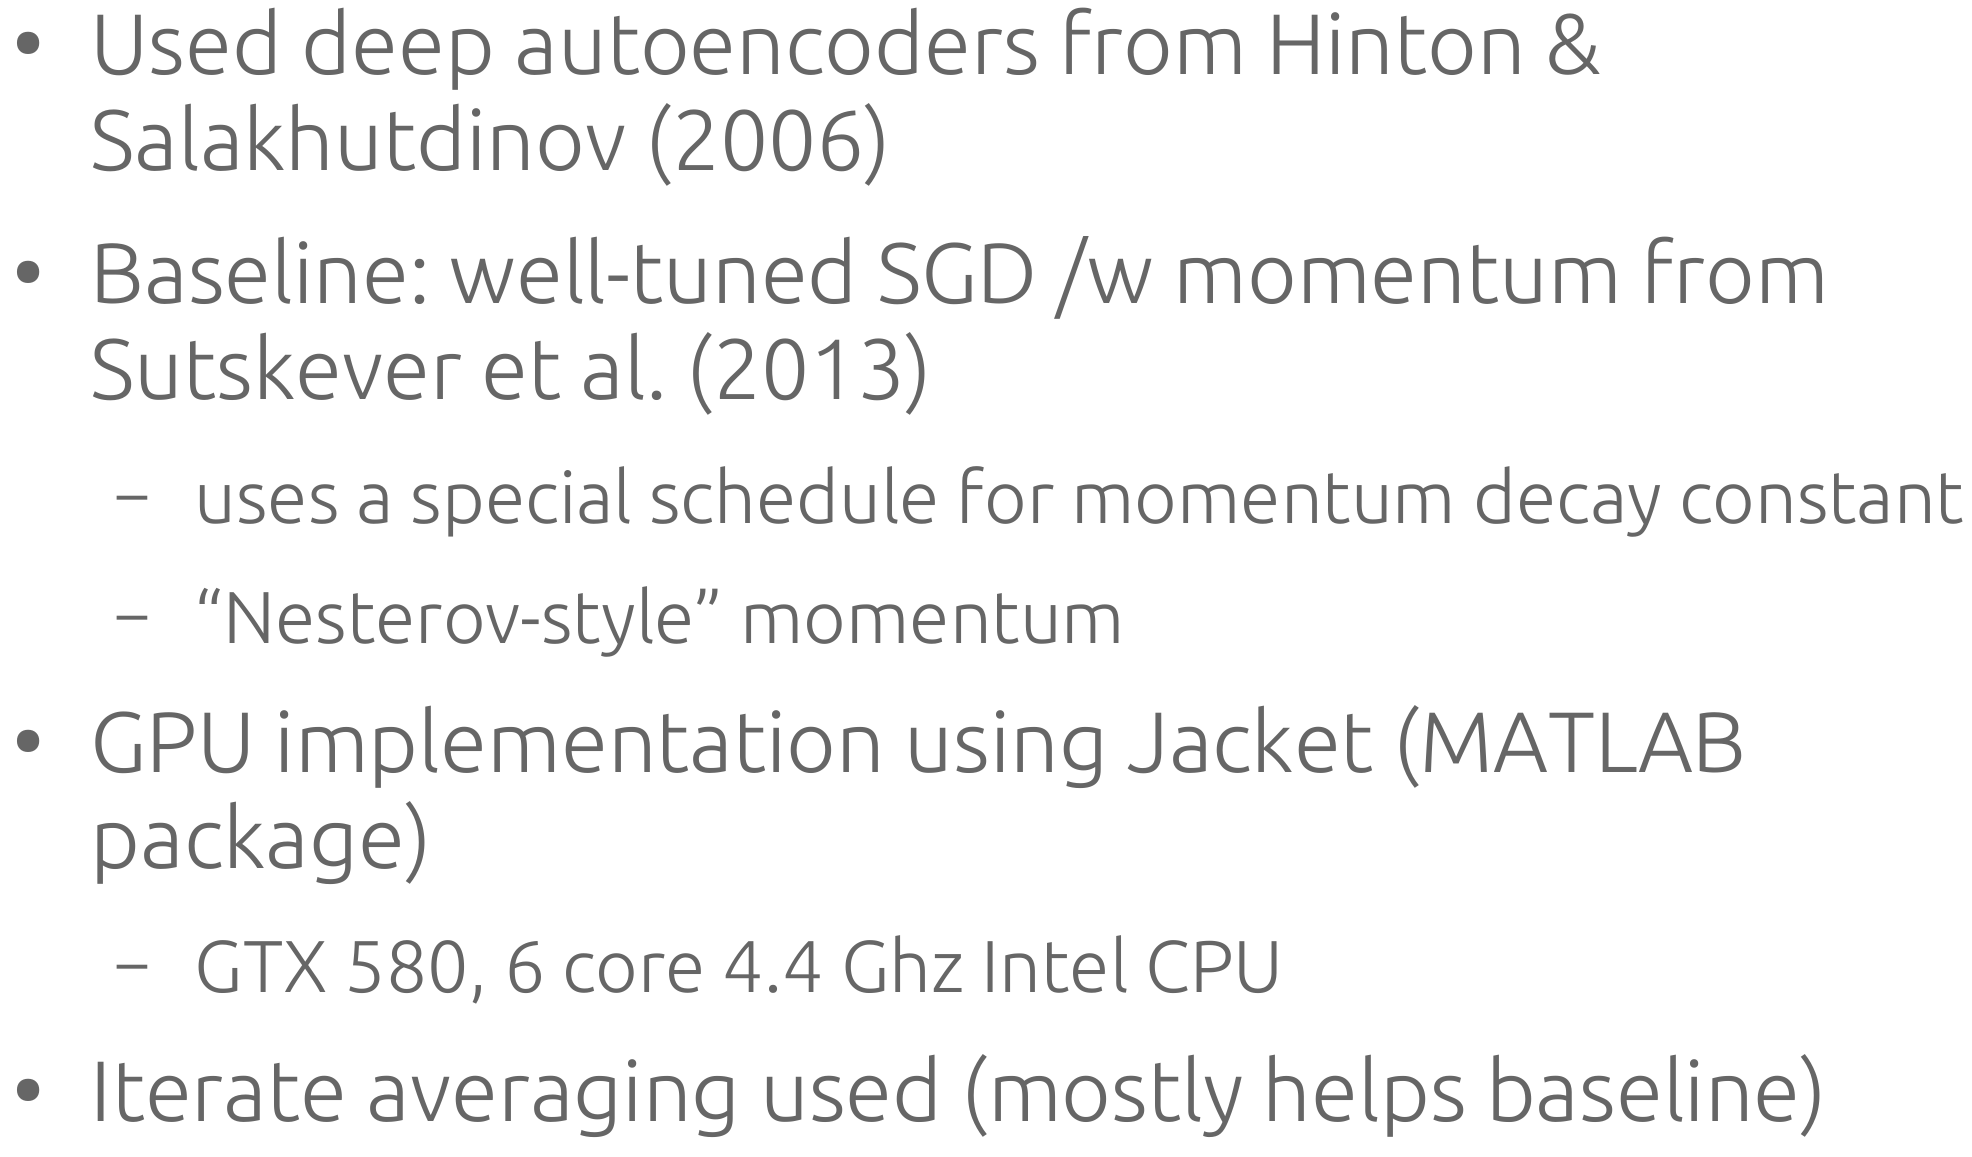
\includegraphics[scale=0.225]{xprmt_setup}
% \end{figure}
\end{frame}

\begin{frame}
\frametitle{Experiments}
\begin{figure}
    \centering
    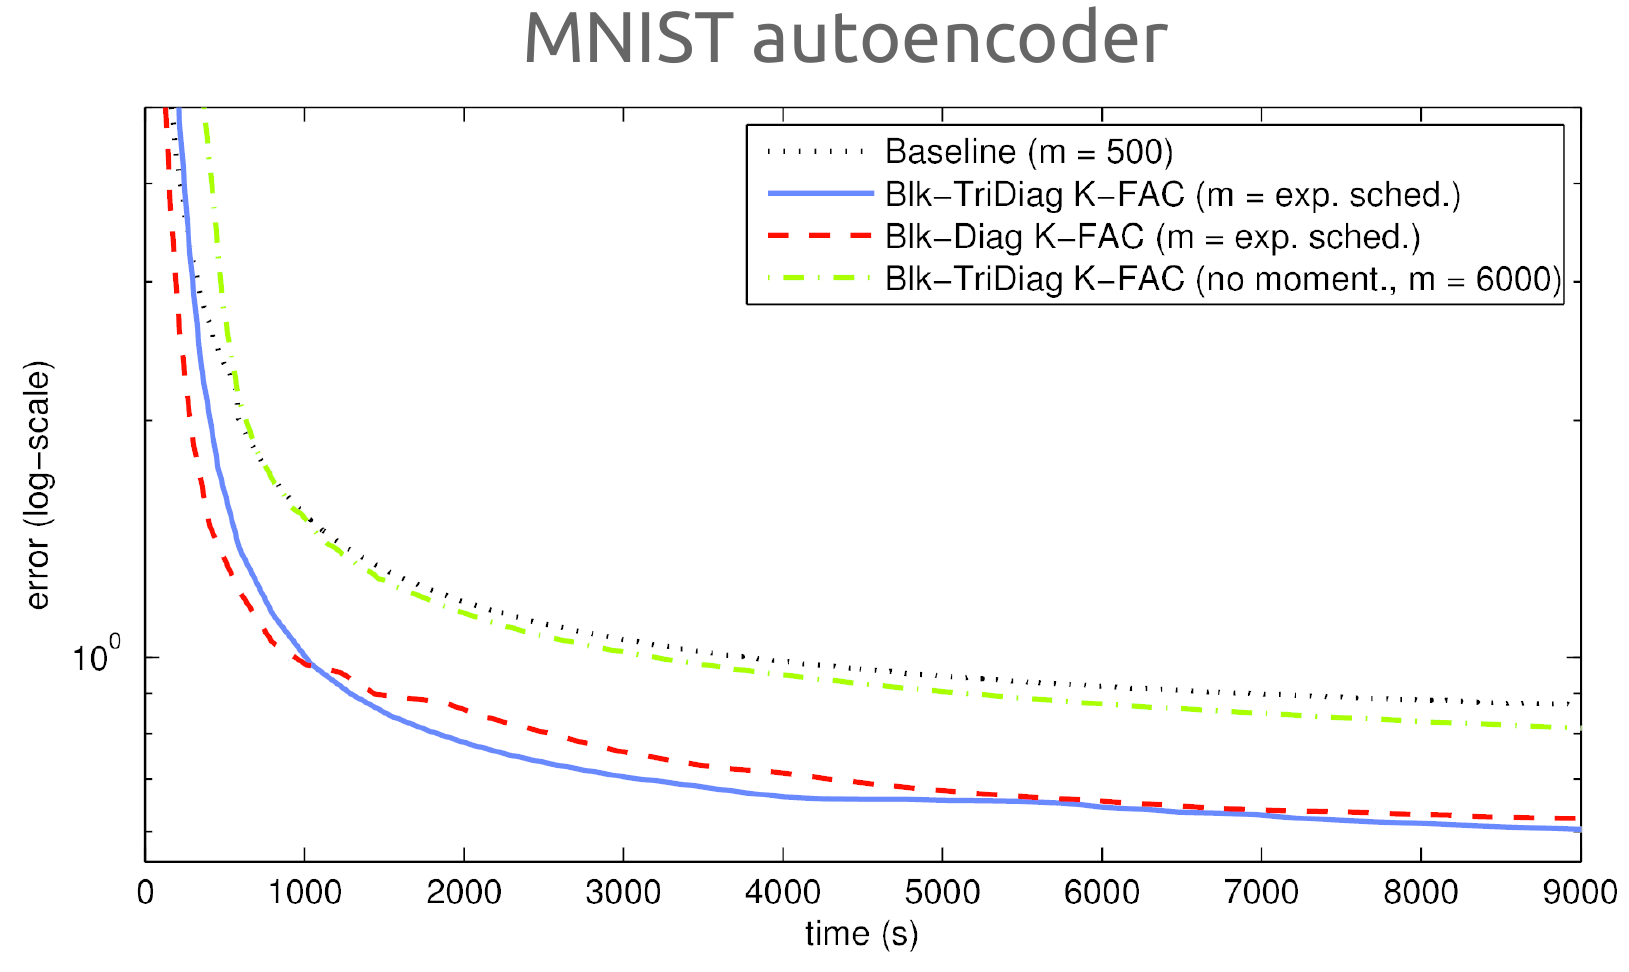
\includegraphics[scale=0.275]{mnist_autoencoder}
\end{figure}
Note: momentum and minibatch size scheduling are crucial!
\end{frame}

\begin{frame}
\frametitle{Experiments}
\begin{figure}
    \centering
    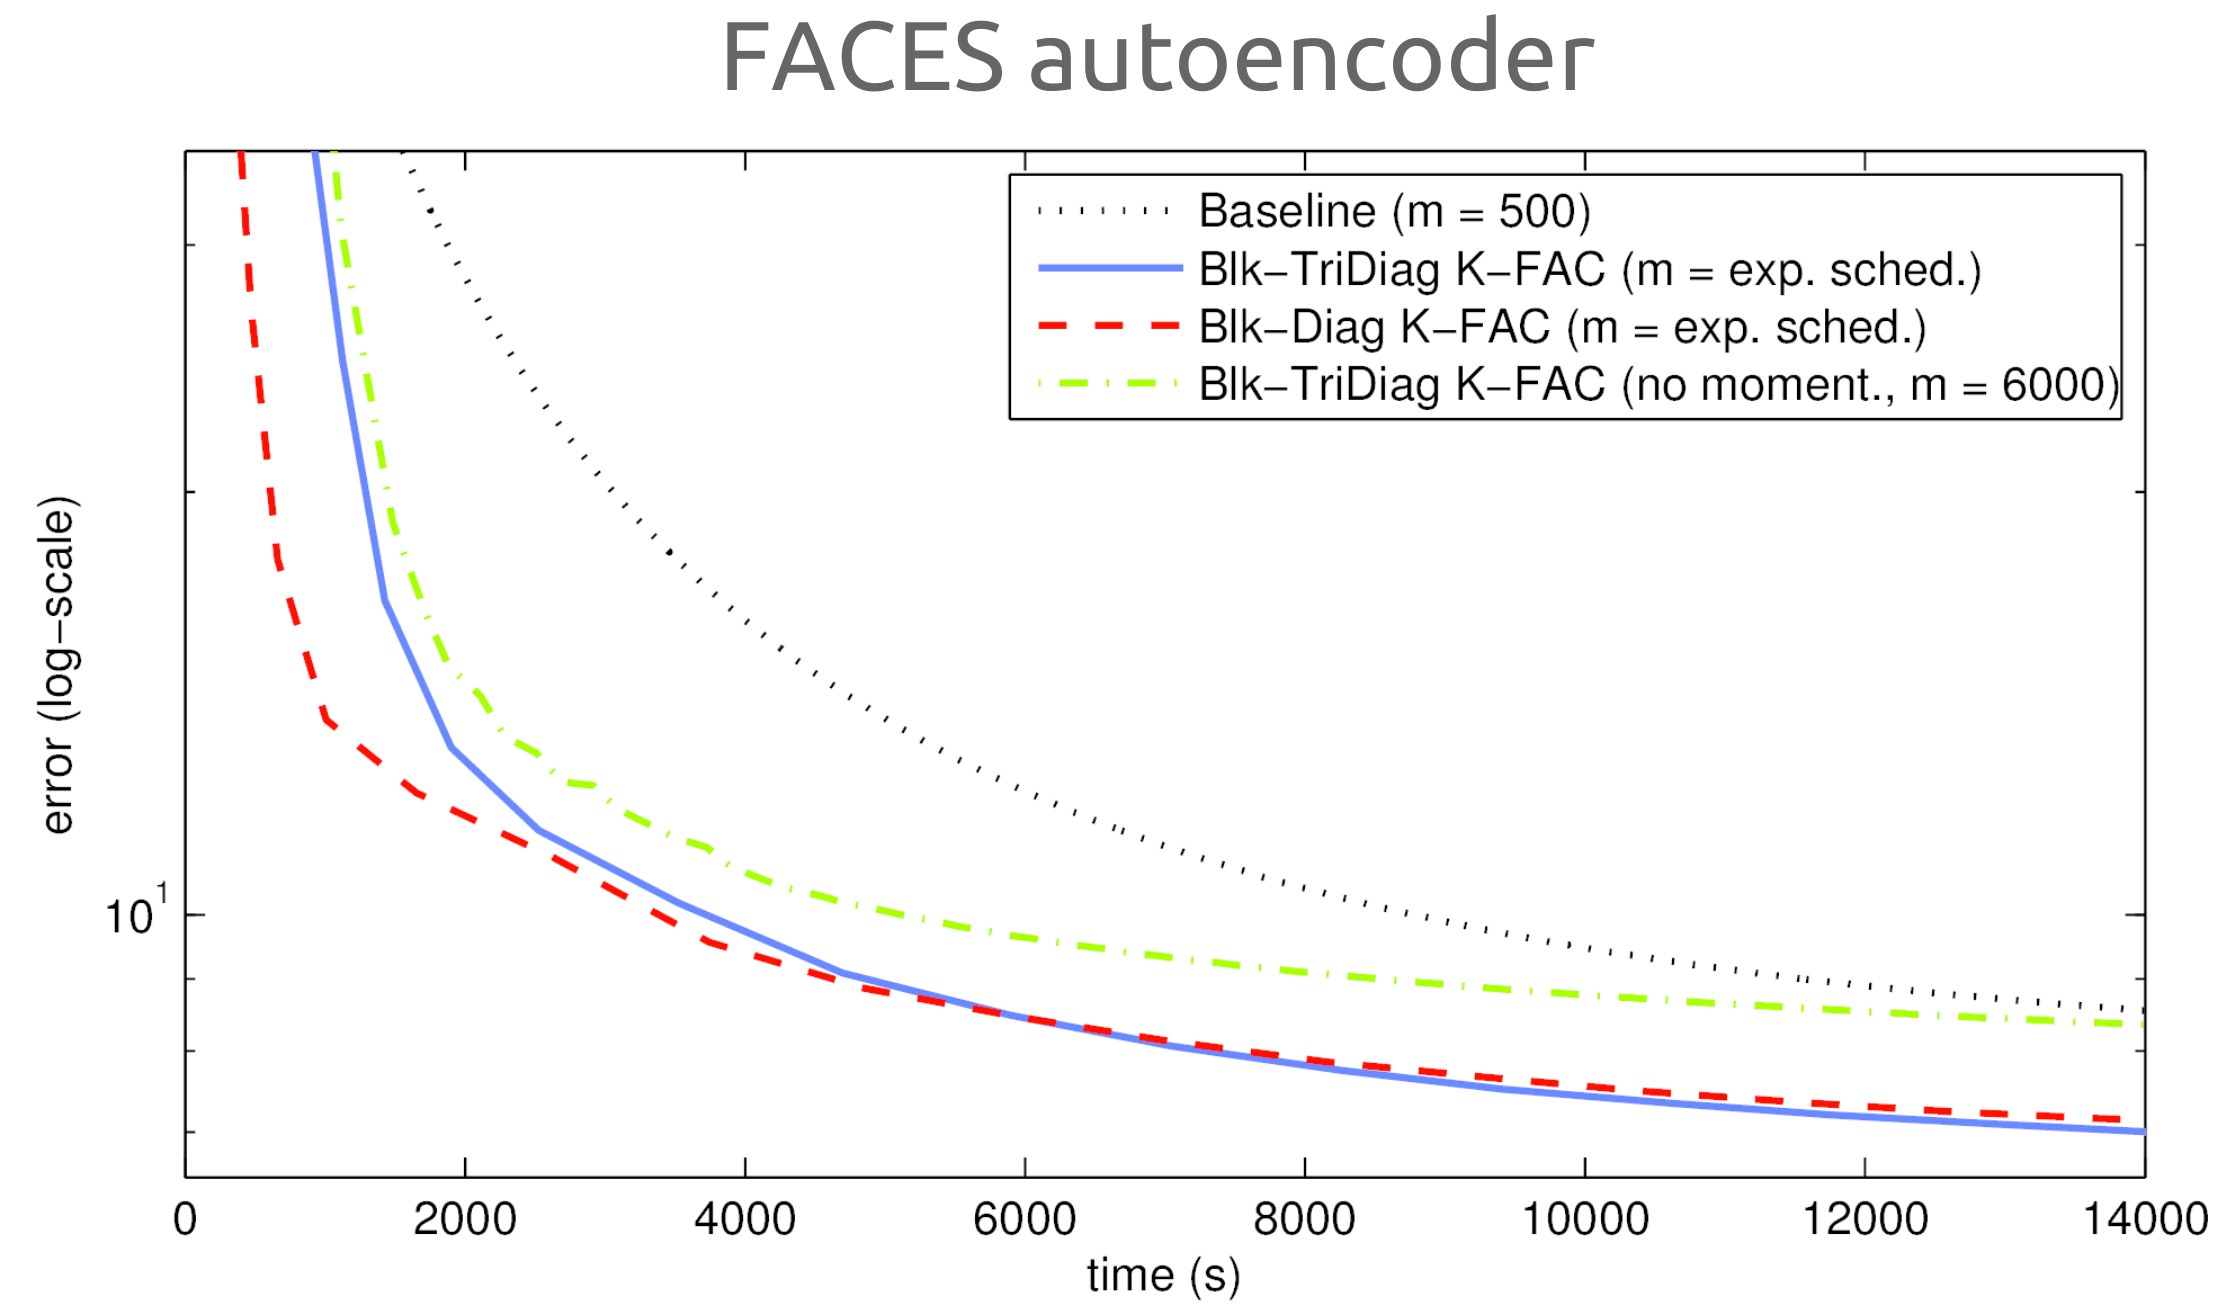
\includegraphics[scale=0.175]{faces_autoencoder}
\end{figure}
Note: the block-diagonal approx is good enough already :), \\
compared to the more sophisticated block-tridiagonal approx!
\end{frame}
